\chapter{Introduction}\label{C:Introduction}
%%require: strong-motiv, clear-focus, induce-logic
%%require: fig, data, trends
%%require: cs-wireless-intro, general apps.
%%require: good history

\indent \indent This chapter firstly introduces the challenges in signal processing with respect of signal acquiring limitation due to Nyquist sampling theorem, and then turn to focus on the compressed sensing (CS) for solving the problem. Next, potential CS based wireless applications, especially those for wideband signal processing, are proposed. Besides, it is still important to point out that there still exist several gaps between CS theory and its hardware implementations involving constraints like energy-cost, non-ideal model mismatch, real-time capacity. These gaps motivate our investigations and future research. At last, the organisation of the entire report is presented.

\section{Challenges of Signal Processing}
\indent \indent Signal processing is to processes or transfers information that contained in real world signals. The principle of signal processing is firstly founded by Alan V. Oppenheim and Ronald W. Schafer, and so far widely developed and related to modelling, analysis, extraction, learning, security etc \cite{moura2009signal}. 

Once Oppenheim and Schafer stated that the "digitisation" can be applied in signal processing \cite{oppenheim1989discrete}, signal processing is tightly linked with digitisation, for it can provide additional benefits such as compression and error detection \cite{broesch2008digital}. Consequently, the digital signal processing (DSP) algorithms and devices have been widely deployed in image processing, video conferencing, smart sensors network, and other real-time processing tasks. Its applications are also increasingly implemented in the form of embedded systems such as mobile and wireless devices\cite{mamaghanian2011compressed}, aerospace equipment, and biomedical instruments\cite{lustig2008compressed}.

However, during the digitisation, signal acquiring and quantification are always highly restricted by the sampling rate, because the famous Shannon theory states that the minimum sampling rate should be at least twice as the most highest frequency components of original signals (we also call it the Nyquist rate). As a result, DSP devices have to match the high sampling rate requirements in their input front-end. What's worse, because the input front-end of DSP is the first stage of the entire system, the limitation of sampling rate correspondingly influences the further stages for data processing and storage.

Therefore, the limitation in signal sampling not only increases the design complexity to analog-to-digital converters (ADCs), which is the input front-end of DSP, but increases the data size of storage, as well as the scale for further data processing. Consequently, the power consumption, computational cost, and commercial design cost become raising. What's worse, as the trend of developing DSPs requires faster sampling, larger dynamic range, higher dimensional data, low-energy consumption and high sensing mobility \cite{danckaert1999strategy}, if we cannot solve the sampling limitation, then not only sampling itself, which relates to faster sampling, larger range and sensing mobility, but also burden storage for high dimensional data and energy saving for low-energy consumption, will be significantly affected. In one word, all requirement refers to the key problem of sampling. From this aspect, solving the limitation in signal sampling is by no means tolerable for modern signal processing devices.

\section{Compressed Sensing Overview}
\indent \indent Fortunately, the compressed sensing (CS) presents us an useful approach to extract sparse interests of signal BELOW the Nyquist rate. The CS framework provides high possibility to reconstruct original signals through few randomly sampled data than traditional Nyquist sampling method. Using the l1-norm minimisation, figure \ref{I:intro-cs} demonstrates the recovery results between CS reconstruction and conventional recovery. From the comparison, we can conclude that the CS successfully recover the sparse spectrum information from the original signals. The following paragraphs presents related topics for CS. 

\begin{figure}
\label{I:intro-cs}
\centering
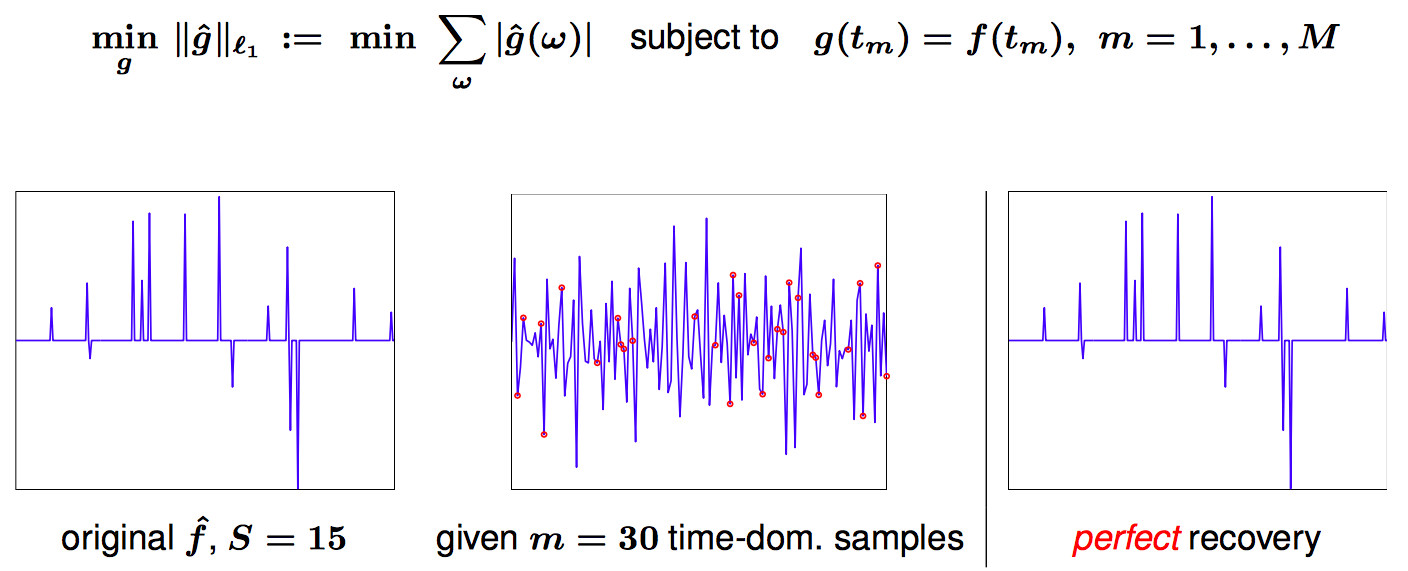
\includegraphics[width=5.0in]{figs/cs-reconst-intro.png}
\DeclareGraphicsExtensions.
\end{figure}

\paragraph{Sparsity}
The goal of signal processing is to reconstruct the original signal from a stream of samples. In the procedure of reconstruction, fewer samples of information is needed if the prior knowledge of signal’s frequencies is clear. By appropriate representation, e.g. Fourier basis representation, natural signals are always represented by few significant coefficients, and termed as sparse information. Mathematically, the sparse information can be presented if assuming the signal of $x \in R^N$ can be decomposed by a group of basis $\Psi$, where $k << N$:  
\begin{equation}
x=\Psi s=\sum_{l=1}^{K}\psi_l s_l  
\end{equation}
Here $x$ is a linear combination of $K$ basis chosen from $\Psi$, and $s$ is the corresponding coefficients of representing $x$ in the domain constructed by the basis $\Psi$. 

\paragraph{Incoherence}
The incoherence presents the idea that signals $x$ containing a sparse representation in basis $\Psi$ must be spread out in the basis domain in which they are acquired \cite{candes2008introduction}. For instance, the spike is spread out in the frequency domain. In other words, the incoherence indicates the sampling/sensing waveforms have an extremely dense representation in the basis. 

\paragraph{Relevance}
Similarly, the wavelets compression \cite{chui1992introduction} e.g JPEG2000 also develops the sparse information in natural images. It represents images into approximately sparse and ignores large amount of small (nearly zero) coefficients. This is the reason why the wavelets only remain small size data while keeping the image with high information. For instance, using wavelets, natural images can be compressed into a relative small size ( < 5 percent of original size) while still keeping high quality. An example is demonstrated in figure \ref{I:wavelet-intro}.

\begin{figure}
\label{I:wavelet-intro}
\centering
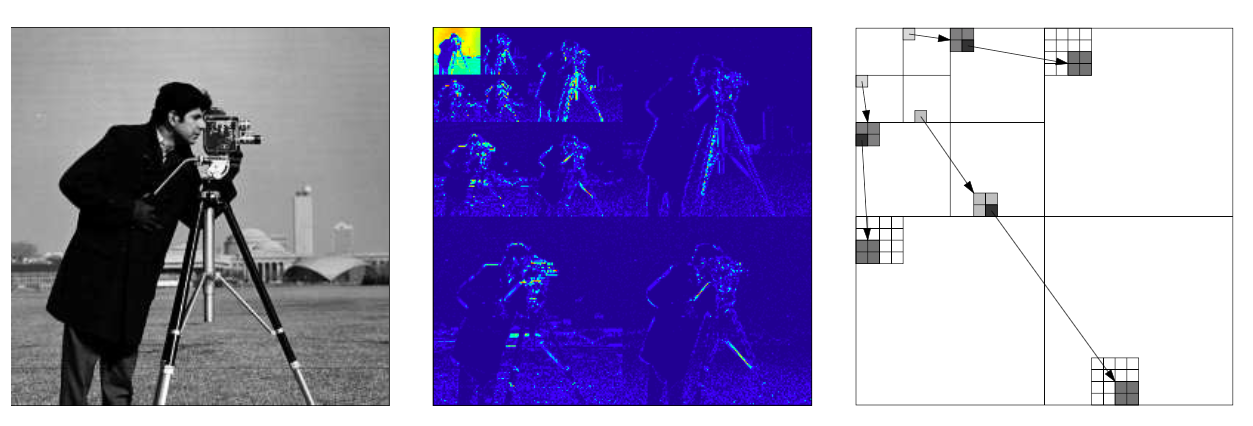
\includegraphics[width=5.0in]{figs/wavelets-intro.png}
\DeclareGraphicsExtensions.
\caption{An example of Haar-wavelet decomposition. Only light coefficients are significant. Dark ones are nearly zero and can be neglected.}
\end{figure}

According to the principles of wavelets, the steps of this approach can be described as sample then compress. However, in the step of sampling, the Nyquist rate is still required. This is the main difficult between CS and wavelets, since the CS can overcome the limitation provided by the Nyquist rate. 

\paragraph{Develop of CS}
Around 2005, Terence Tao, David Donoho, Emmanuel Candès mathematically proved that using random selection, the low-rate sampled measurements can reconstruct original data with high possibility, using $l1$-norm minimisation \cite{candes2006robust,baraniuk2007compressive} shown as equation \ref{eq_l1_min}. 
\begin{equation}
\label{eq_l1_min}
\hat s = \arg\min \| s \|_1 \quad s.t. \quad  y = A s
\end{equation} 
, where it has been proven that only $O(K\ln(N/K))$ samples are needed if matrix $A$ are incoherent with $s$. One of the best choice for the independence is to use i.i.d variables (independent and identically distributed variables) constructed matrix such as the Gaussian matrix. Further, more constructed matrix like Bernoulli matrix, partial Fourier matrix are proven suitable for CS. Therefore, CS provides a novel random sampling paradigm which is applicable for modern signal sampling and data processing with low rate. 

\section{Typical Compressed Sensing Applications}

\paragraph{Compressive Radar Systems}
Compressed sensing has showed outstanding feature in  in reducing the sampling rate in many wireless applications, e.g. radar systems, since many wireless devices communicate at high frequency which lead to heavy burden in sampling task so that the CS can be used to reduce the sampling rate at receivers \cite{bajwa2006compressive}. In addition, in radar systems, it's necessary to have capacity to acquire wideband signals with different signal templates, such as TV bands, satellite signals, cell-phone informations etc. Traditional method always require filter-banks to down-sample these signals, while the CS can help original system directly sense the various of wide-band signal, or with less filters. The figure \ref{I:cs-radar-intro} presents a wide-band signal monitoring and processing radar system that receives signals from a variety of sources.

\begin{figure}
\label{I:cs-radar-intro}
\centering
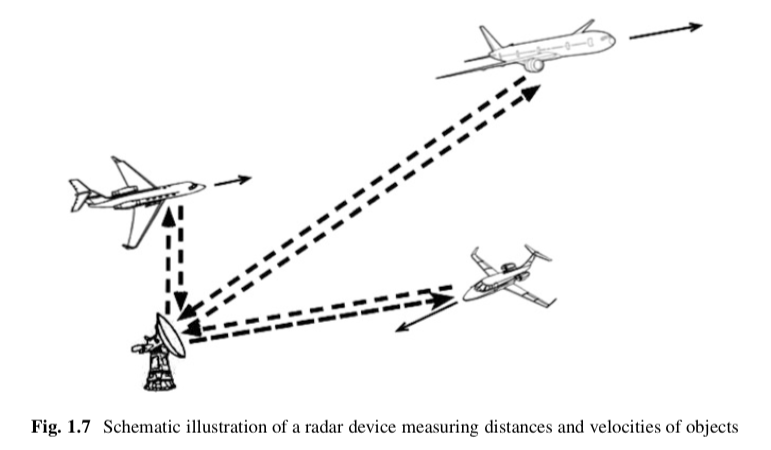
\includegraphics[width=5.0in]{figs/cs-radar-intro.png}
\DeclareGraphicsExtensions.
\end{figure}

\paragraph{Compressive Single Pixel Camera}
Different from the wavelets, compressed sensing requires little samples which reduce the energy during image acquisition. For instance, the CS framework is implemented for single-pixel cameras by  Rice University \cite{baraniuk2008single}. This new CS-camera directly acquires random projected samples from a image without first gain the pixels, and the random projected samples are collected by digital micro-mirror array, which optically reflects a linear projection of the image onto pseudo-random binary patterns.

\begin{figure}
\centering
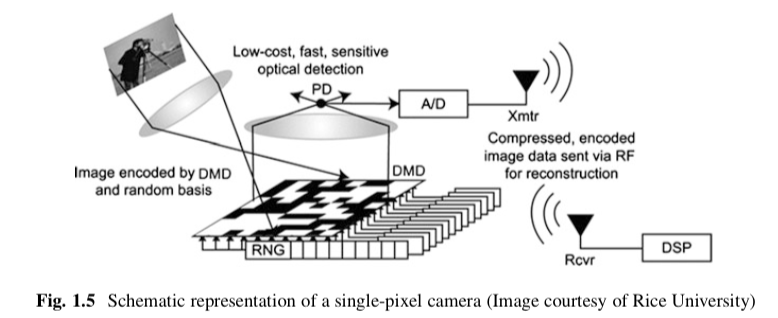
\includegraphics[width=5.0in]{figs/cs-camera-intro.png}
\DeclareGraphicsExtensions.
\end{figure}

\paragraph{Magnetic Resonance Imaging}
Magnetic resonance imaging (MRI) is a widely used technology in medical imaging, applications such as brain scanning, angiography, and dynamic heart imaging are necessary for medical diagnosis \cite{foucart2013mathematical}. However, this imaging tool burdened by an inherently slow data acquisition process since traditional approaches based on the Shannon sampling theorem requires long-time scanning if the high-resolution images are required \cite{lustig2007sparse}. In the cases that the patients cannot be expected to hold statically for long-period (e.g. children are too impatient to sit for more than minutes). The embedding CS to MRI has the potential to significantly reduce the scan time. 

\begin{figure}
\label{I:cs-mri-intro}
\centering
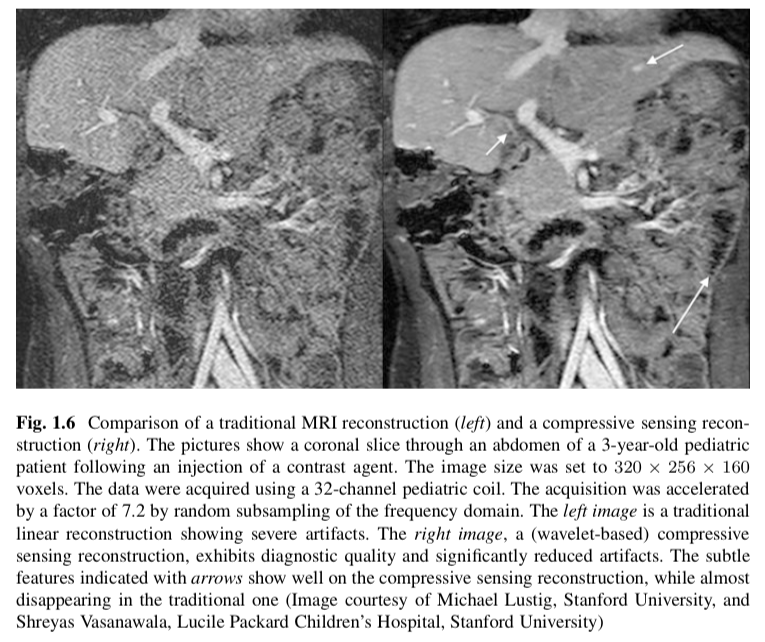
\includegraphics[width=5.0in]{figs/cs-mri-intro.png}
\DeclareGraphicsExtensions.
\caption{The comparison of a traditional MRI reconstruction (left) and a compressive sensing reconstruction (right).}
\end{figure}

\section{Compressive Wireless Communication}
\indent	\indent Over the past few decades, the demand for high frequency communication and wideband signal detection keeps increasing, which worsen the acquiring the situation. For instance, modern digital systems often require bigger data size, or higher rate communication (e.g. ultra-wideband), or more flexible networks (which emerges hybrid wireless devices, e.g. cognitive radio), and all the requirements highly rely on accurate and sensitive sampling approaches. Thus, enhancing the performance of sampling devices brooks no delay. 

Therefore, our study motivation derives from the problem of signal acquisition devices, especially for those who aims at collecting wideband / high frequency signals. An suitable research object is the wireless application, for many applications are communicating at high frequency, and becoming more and more depend on high performance receivers and detectors, as well as the novel sampling approaches. Fortunately, the compressed sensing (CS) presents us an useful approach to extract sparse interests of signal BELOW Nyquist rate. This novel approach motivates a large range of application in signal processing. The next section will introduce this method. 

In fact, although the CS framework solve the problem in Nyquist sampling rate theoretically, the gap between hardware applications and ideal cases still remain. For instance, as the CS theory often requires a true randomness in sampling approaches, while hardware implementations only provide pseudo-randomness instead. The constraints doesn't only stay in CS theory implementation, but design limitations or awareness such as energy consumption, real-time capability, design complexity etc. All the constraints bring about tradeoffs design schemes, so CS applications for wireless, signal processing is still an open issue. 

\subsection{Research Aims}
\indent \indent As an important application area for CS, wireless communication is always puzzled by high frequency transmission detection or wideband signal processing, e.g. radar systems. Those applications, to our best knowledge, are mainly focus on high frequency required scenarios, including multiple-input and multiple-output (MIMO), multiple access (MA), ultra-wideband (UWB), cognitive radio (CR).

In this report, we are more focusing on CS based wireless communication, especially aims at the physical layer and MAC layer. For research applications, we select two typical and popular applications, which  involves extremely high-frequency and wide bandwidth signal processing respectively -- the ultra-wideband  system and cognitive radio. 

\paragraph{Compressive Ultra-Wideband Positioning} 
The Ultra-Wideband (UWB) communication is widely used in wireless communication and associated with features as extreme wide transmission bandwidth, low-power consumption, shared spectrum resources in wide ranges etc. However, for many ultra wideband communication systems, how to energy-efficiently collect signals higher than GHz is a crucial problem. In order to solve these problems, we study the novel approach that embeds CS into the UWB positioning. In our proposed compressive UWB positioning system, random projection is located at transmitters to support CS framework while sub-Nyquist low-rate ADCs are implemented at receivers. As a result, not only the accuracy is improved but also the sampling cost is significantly reduced. The detailed design is introduced in chapter \ref{C:compressive_uwb_positioning}.

\paragraph{Compressive Cognitive Radio Spectrum Sensing}
Cognitive Radio (CR) has been attracting many attention due to its potential better utilisation for limited spectrum resources. However, for many cognitive radios, how to accurately and quickly sense the occupation of active primary users (PUs) without additional interference is a crucial problem. In order to solve this problems, we study the novel approach in chapter \ref{C:wideband_css} embedding CS into recent CR spectrum sensing techniques. Then we analyse the performance and cost for applying the CS. The analysis and discussion finally motivates us for future research on compressive signal processing (CSP) for cognitive spectrum sensing in chapter \ref{C:csp_css}.

\section{Problem Statement}\label{sct:problem_state}
\indent \indent In this chapter, we narrow the concerned problems to CS wireless hardware designs, mainly from two aspects: (1) Although the CS is outstanding for its significance in reducing the sampling rate, however, as a sacrifice, the reconstruction procedure is non-linear and full of complexity and difficulty. (2) Besides, CS sensing model hardware implementation is not easy and simple, for building absolute incoherent and independent sensing matrix is challenging (e.g. true randomness in Gaussian matrix can hardly be implemented in computer engineering field). The following problems open up some interesting issues for our research, and  some of them are focused in this report and some will be studied in our future works. 

\paragraph{Real-Time Capability}
The reconstruction algorithms for CS is non-linear, which indicates that the recovered data are not directly suitable for conventional digital signal processing where a simple linear recovery using cardinal sine interpolation is needed. Besides, some of the high accuracy reconstruction algorithms based on convex optimisation are time consuming, e.g. the basis pursuit's complexity is $O(N^3)$, which generates large time delay for further data processing, and do harm to the feed-back required devices. On the other hand, even though greedy method (e.g. the orthogonal matching pursuit's complexity is $O(kMN)$) has speed up the sunning time for CS reconstruction, the recovered data is located in different domain, e.g. original data is sampled in time domain while the recovered data in frequency or spatial domain. The domain mismatch sometimes require addition transforming task which generates more cost in time and energy. In one word, CS reconstruction make the real-time capability worse, and lead many CS techniques not suitable for feed-back required processing systems.  

\paragraph{Processing Flexibility}
Higher flexibility is one of the important trend and requirement for modern signal processing devices. In contrast to the task-specific hardware used in many classical acquisition systems, many hardware designed to use a compressive measurement protocol can be extremely flexible. 
A stylised future CS radar system demonstrate the potential signal processing pattern for wide-band signals:  In figure \ref{I:cs-radar-intro}, the CS radar receives various types of signals from televisions, cellphones, aeroplanes and satellites etc. However, the signals' templates are unknown to the system, such as signal-to-noise ratio and sparsity order which seriously affect the performance of detectors. Then what information should be collected ? How to accomplish matched filters ? Is adaptive selection needed ? These solutions sometimes computational expensive but not flexible enough. What's worse, the CS reconstruction is non-linear which does not match the traditional processing approaches and thus increase the analysis difficulty. 

\paragraph{Energy Efficiency}
Compressed sensing community has provided many hardware architectures for analog-to-digital information to build sub-Nyquist rate analog-to-digital converters (ADCs), such as random demodulator (RD) \cite{tropp2010beyond} and modulated wideband converter (MWC) \cite{mishali2009expected} mentioned in chapter \ref{C:compressed_sensing}. In facts, however, most CS based ADC architectures do NOT eliminate  Nyquist rate in entire systems -- although the sampling rate reduced, the mixing rate for random projection remains Nyquist rate. Besides, some CS framework involves random filtering, however, the randomised coefficients for filter's impulse response is hard to implement. In addition, aforementioned CS non-linear reconstruction cost still suffers the entire system in energy consumption. Therefore, concerning the design complexity and energy cost and correspondingly making acceptable tradeoffs is a necessary topic.  

\paragraph{Sensing Matrix Construction}
Different from the Nyquist sampling approaches which samples at uniform time grid, the compressed sensing framework acquires data relying on the inner product \cite{laska2011polyphase}. Consequently, the different sampling approach generates different implementations in ADC design. However, the CS sensing model hardware implementation is not easy and simple, since building absolute incoherent and independent sensing matrix is challenging. For instance, true random variable comprised sensing matrix can hardly be implemented in computer engineering field. Consequently, approximations for CS theory to CS implementation are often required, such as using pseudo-randomness, or using less independent sensing matrix etc. As a result, the non-ideality of the sensing sampling in hardware design generates in-negligible errors. 

\section{Major Contributions}
\indent \indent This report studies novel energy-aware and real-time ability improved approaches for embedding the CS framework into cognitive radios (CR) and ultra-wideband (UWB) systems. The brief introduction about the contributions are shown as follows:

\paragraph{Implementation for energy-aware design in compressive UWB positioning} 
The compressed sensing is proven effective to improve the accuracy of IR-UWB positioning. However, most of papers do not concern the design complexity and energy cost in their implementations, for instance, the random mixing waveform is of extremely high frequency (in GHz). Our proposed compressive UWB positioning present a novel view of energy trade-off design, which is implemented by a low-rate random-projection at transmitters and low rate ADCs at receivers. It is clear that this design significantly reduce the peak frequency in the system with only acceptable rate increase in receivers' ADC sampling rate. 

\paragraph{Exploration for direct signal processing in compressive detector in CR} 
The compressed sensing does not directly match the traditional processing algorithms (section \ref{sct:problem_state}). However, in cognitive radio, most of tasks for spectrum sensing are related to detection, estimation, filtering, classification. This contradiction leads the large additional loss in energy usage and time utilisation when we applies the CS to reduce the sampling limitation in wideband sensing for CR. Then noticing the fully reconstruction is always not needed, we discuss the future direction in directly processing compressively sampled data in CR, which aims at extracting effective information without fully recovery so that the entire real-time capability and energy efficiency will be significantly increased. 

\section{Organisation}
\indent \indent The main idea of the research work is to further extend the CS based techniques to wideband signal processing systems for wireless communication, in order the solve the limitation of the sampling rate. Using this approach, a novel CS-based framework for signal processing will be proposed that encompass various areas such as data compression, data acquisition, data storage, data transmission optimal recovery and processing, and also targeted for embedded deployment. In addition, since embedded signal processing system are popular and suitable in many wireless network applications such as battery supplied mobile devices for wireless communication. The rest of this report is organised as follows:

Chapter 2 firstly presents the overview of compressed sensing theory and its applications, and then focuses on wideband signal acquisition hardware design which relates to our survey for recent CS-ADC architectures. Then the following chapter 3 presents our related work in compressive UWB positioning systems. What’s more, the chapter 4 introduces the compressive spectrum sensing for cognitive radios, but points out the limitation due to CS fully reconstruction. Finally, the chapter 5 proposes our recommenced future research on compressive signal processing based cognitive spectrum sensing.

%\begin{itemize}
%  \item \textbf{Chapter \ref{C:compressed_sensing}} presents the overview of compressed sensing theory and %its applications, then focus on wideband signal acquisition which relates to our survey of CS-ADCs design.  
%  \item \textbf{Chapter \ref{C:compressive_uwb_positioning}} presents an overview in ultra wideband (UWB) %systems. Especially, our proposed CS-based potential technique, which produces a trade-off between random %mixing rate and sampling rate, is introduced for ultra wideband positioning. 
%  \item \textbf{Chapter \ref{compressive_css}} analyses the performance and features in CS-based cognitive %spectrum sensing (CSS), and propose our recommenced future idea on directly extracting features from %compressed measurement for cognitive radio (term as compressive signal processing, CSP).
%\end{itemize}

%  \indent \indent Visual surveillance system is a smart system that assists humans to extend perceptions and capability in monitoring interesting areas \cite{regazzoni2001special}. With surveillance systems, interesting situations would be automatically detected and analysed, which breaking the area limitation of human perception and reducing labour cost in surveillance.
%  
%  Surveillance systems now have been widely used in multiple applications as shown in Figure \ref{fig:SurveillanceApp} : (1) safety in transport applications \cite{regazzoni1998advanced,foresti2000multimedia} like monitoring of urban and city road conditions \cite{roller1993model,boyd1999statistical,blosseville1999image}, motorways dangerous events alert \cite{foresti1999monitoring}, maritime environment surveillance \cite{sanderson1997target,ince1997design,olsen1995operational}, and airport guidance and control \cite{lynn1993application,galati1995advanced,braasch2000laas}; (2) public security for people in places of buildings \cite{lin1998building,vergara2000automatic}, car parks \cite{cattle1995use}, banks \cite{bederson1992miniaturized}, etc; (3) military applications like air surveillance \cite{draper1999tracking,van1999aircraft} and enemy movements in battlefield \cite{peters1998sensor,fennell1998battlefield}; (4) human activity analysis \cite{haritaoglu2000w,hongeng2000representation,gavrilla1999analysis,oliver2000bayesian,galata2001learning,freer1997automatic}.
%  
%  \begin{figure}
%    \centering
%    % Requires \usepackage{graphicx}
%    \includegraphics[width=0.95\textwidth]{SurveillanceApp.eps}\\
%    \caption{Different surveillance system applications}\label{fig:SurveillanceApp}
%  \end{figure}
%  
%  There have been a lot of successful surveillance programs/projects carried out by different groups for the tasks of public/pravite security. The United States Department of Homeland Security Threat and Vulnerably Testing and Assessment (TVTA) portfolio involves an project of ADVISE (Analysis, Dissemination, Visualization, Insight and Semantic Enhancement). This ADVISE project is reported as a data-mining project which rely on personal data to track individual behaviour \cite{ADVISE2007}. This system focuses more on high level tasks like behavior analysis and information synthesis based on large data from different sources.
%  
%  IBM released their smart surveillance system "IBM Smart System Surveillance Solution" \cite{hampapur2004s3} in 2004. This smart surveillance system provides the capability to automatically monitor a scene by a number of video analysis techniques like object detection, tracking and classification. Beyond the detection and tracking level, the IBM smart surveillance system also provides the capability to manage the surveillance data, perform event based retrieval, receive real time event alerts through standard web infrastructure and extract long term statistical patterns of activity.
%  
%  In 2010, Google has tested their driverless car system in several vehicles for 1,000 miles without any human intervention, in addition to 140,000 miles with occasional human intervention \cite{thrun2011google}. The system can handle different scenarios like streets in the city, highways, mountain roads, even night driving and etc. This system is expected to help reduce the number of traffic-related injuries and deaths, while using energy and space on roadways more efficiently. In such driverless car systems, a surveillance-like system is embedded to modify the surroundings and helps make decision to the vehicle control system.
%  
%  There are also other programs like Annotated Digital Video for Surveillance and Optimized Retrieval (ADVISOR) sponsored by the European Union. This program is excepted to be used in surveillance for public transport and metro network \cite{siebel2004advisor}. In 1997, the Defense Advanced Research Projects Agency (DARPA) Information Systems Office started a three-year program to develop Video Surveillance and Monitoring (VSAM) technology, an automated video understanding technology for use in future urban and battlefield surveillance applications \cite{davis1998visual}. In UK, the University of Reading has developed the VIEWS system for traffic management \cite{hu2004survey}. All the above systems are regarded as visual surveillance systems in different applications.
%  
%  For the past 50 years, researches in surveillance system can be divided in to 3 stages -- 1GSS (First generation video surveillance systems), 2GSS and 3GSS \cite{regazzoni2001special}, the architectural examples of 1,2,3GSS is given in Figure \ref{fig:1_2_3GSS}.
% 
% \paragraph{First generation video surveillance systems (1GSS)} (1960-1980) was developed to extend the human perception capabilities in spatial sense. Multiple analog cameras are installed at difference interested regions. There are less artificial intelligence techniques in the 1GSS. The major limitations of 1GSS are due to the restrictions in analog signal processing and transmission level: large bandwidth requirement for number of sensors \cite{pahlavan1994wireless}; image quality decline subject to noise in transmission \cite{sacchi1999remote}; difficulties in significant event signal retrieval due to the storage medium of taps.
% 
% \paragraph{Second generation video surveillance systems (2GSS)} (1980-2000) benefited a lot from the digital signal processing techniques. In this stage, more efforts had been put in real time automated interest event detection and recognition. And the research studies focus on areas like object recognition and tracking \cite{foresti1998object,marchand1999robust,lowe1992robust}, human behavior understanding \cite{haritaoglu2000w,hongeng2000representation}, intelligent human computer interface \cite{haanpaa1997advanced}, digital signal processing for video compression \cite{bjontegaard1996comparison,cheng2000partial}. But in 2GSS, surveillance system research was still limited to local area with CCTV (Closed Circuit Television) camera networks \cite{kim2010intelligent}.
% 
% \paragraph{Third generation video surveillance systems (3GSS)} (2000-now) is based on full digital signal processing techniques. The sensors are so-called intelligent cameras and the local processing layer is able to compress the digital signal to save bandwidth. Comparing the CCTV camera networks used in 2GSS, 3GSS introduces the intelligent hub in the network layer, which enable different communication mediums (like wireless, cable, network access, etc.) of the local processing layer. Besides, the researches on interest event detection and recognition are still developing \cite{bevilacqua2006high,foresti2003robust,hager2004multiple,kalal2012tracking,iVT2008,breitenstein2011online}.

% \begin{figure}
%   \centering
%   % Requires \usepackage{graphicx}
%   \includegraphics[width=0.98\textwidth]{1_2_3GSS.eps}\\
%   \caption{Architecture examples of 1,2,3GSS}\label{fig:1_2_3GSS}
% \end{figure}
% 
% For most of the visual surveillance systems in recent existing projects, the general framework is given in Figure \ref{fig:SurveillanceFramework}. For steady camera input system, the background can be modeled, which is a pre-processing step for better results of object detection and tracking. But usually, the background is dynamic due to the environment changing or PTZ (Pan-Tilt-Zoom) action of the camera. So, the background modeling step is optional. Then, the major task of the surveillance system can be divided into three parts, (1) Multiple camera control and cooperation, (2) object detection and tracking, (3) high level tasks of object behavior analysis, object classification and target identification.
% 
% \begin{figure}
%   \centering
%   % Requires \usepackage{graphicx}
%   \includegraphics[width=0.98\textwidth]{ViSurFramework.eps}\\
%   \caption{General visual surveillance system framework}\label{fig:SurveillanceFramework}
% \end{figure}
% 
% The multiple camera control and cooperation in surveillance systems is for broadening the interest territory. Besides, sometimes the multi-view of the objects given by multiple camera helps in building more robust object appearance model, with 3-D appearance information rather than 2-D in single camera.
% 
% It can be easily seen in Figure \ref{fig:SurveillanceFramework}, the object detection and tracking are the preliminaries for the high level tasks of behavior analysis, object classification, target identification. Also, the information from the high level task can be used to improve the accuracy of detection and tracking. Suspicious targets detection and trajectories analysis make the interest event detection feasible. And we can analyse the target behaviour by its trajectories and the tracking result of each part of the target. Summarizing, robust object detection and tracking algorithm is indispensable for smart visual surveillance system, accurate results from object detection and tracking are significant for the overall performance of the whole visual surveillance system. In this research, we focus on the topic of object tracking in visual surveillance.
% 


%---------------------------------------------------
%\section{Background}
%figures, history

%\section{Challenges in Wireless Signal Processing}

%\indent \indent Signal processing (SP) is to processes or transfers information contained in real world signals such physics, symbolic, or abstract formats. The principle of SP is first founded by Alan V. Oppenheim and Ronald W. Schafer, and so far widely related to modelling, analysis, extraction, learning, security etc \cite{moura2009signal}. Over the past few decades, signal processing (SP) have been developing algorithms for capturing and extracting information from signals, and consequently been widely deployed in image processing, video conferencing, smart sensors network, and other real-time processing technologies. These applications are also increasingly implemented in the form of embedded systems such as mobile and wireless devices\cite{mamaghanian2011compressed}, aerospace equipment, and biomedical instruments\cite{lustig2008compressed} etc.

%Oppenheim and Schafer further stated that the "digitisation" can be applied in the digital control systems \cite{oppenheim1989discrete}. As a result, traditional signal processing utilises digitisation to process data at digital domain quantinized from analog domain, such as measurement, filtering, compression and error detection \cite{broesch2008digital}. Conventionally, the procedure of signal processing is comprised of three steps: 1) quantify analog signal to digital forms using an analog-to-digital converter (ADC), which outputs a stream of discrete digital values. 2) Then the digital signal processor (DSP) produces analysis, filtering or compression to such digital values. 3) At last, some outputs is reconstructed by digital-to-analog converter (DAC) as requirement. 

%The trend of DSP devices are faster sampling, larger dynamic range, higher dimensional data, low-energy consumption and high sensing mobility \cite{danckaert1999strategy}. However, a limitation of signal acquiring is becoming extremely serious, because this limitation affects the first stage (signal acquiring) of DSP, and sequentially influence the following steps of processing and storage correspondingly. This limitation is stated by the Shannon Sampling theory, which declares that the minimum sampling rate should be at least twice as the highest frequency components in original signals. In other words, the higher frequency components exists in original signals, the higher rate for signal acquiring (ADCs) is required, so signal acquiring devices (ADCs) have to match the high sampling rate requirements, which increases the design complexity, energy, and cost. Remark that the signal acquiring is the first stage of DSP, so the entire power consumption, storage size (large number of points needs to be stored), total prize, the processing running time (real-time capability) will also be negatively affected. 

%---------------------------------------------------

%In this report, we are aiming at one of the most crucial limitations lies in the sampling rate (Nyquist sampling rate or Shannon theory, which states the minimum two time sampling rate requirement), which mainly relates to the 1) problem, which also highly influences the 2) and 3) -- Due to limited data processing and storing capability found in many embedded systems, excessive data samples will not only increase heavy burden on data storing and processing/analysing aforementioned in the signal processing procedures, but negatively affect their signal-to-noise performance and power efficiency, and hence forms the bottleneck of entire digital systems. In other words, if we can solve the challenge in sampling rate, we will not only solve the problem of ‘1) acquiring signals at ever higher sampling rates’, but also reduce the data size which affect the problem of 2) and 3), as well as noise and power problems. Consequently, overcoming the sampling rate limitation has become a prevailing research topic, and would be of particular significance for signal processing systems.

%As a novel paradigm for signal processing and acquisition, the compressive sensing or compressed sensing (CS) technique\cite{davenport2011introduction}, is identified to have great potential for resolving the problems mentioned above. The CS theory has been proven to be suitable for numerous computer science and electronic engineering based applications, where it is possible to overcome the limitation of the traditional sampling theory. 

%%fig-cs, rand-signal-sample, recover-suc-rate

%----------------------------------------------------------------------
%———history of CS

%Compressive sensing is a framework that enables the reconstruction of sparse signals from much fewer measurements than the Nyquist rate suggests. CS was introduced by Donoho, Cand` es, Romberg, and Tao in 2006 [1, 2]. This non-adaptive method to acquire measurements directly in a compressed form established a new paradigm in signal processing. Rather than sampling a signal at its Nyquist rate, CS allows to sample at a lower rate, closer to the actual information rate of the signal. This idea has gained significant attention in the research community over the past years. The global research effort in CS is still increasing, not only in information theory, but also in as diverse research areas such as mathematics, computer science, electrical engineering, communications, biology, and even economics. Good introductions to CS can be found in [9], [10], [11], and [12].

%A system acquiring CS measurements can be divided into twoparts. First, compressive measurements are acquired by linear projec- tion onto an incoherent basis. In an ideal case, such measurements are readily available. Otherwise, projections onto an appropriate basis must be performed explicitly. Second, reconstruction recovers the original signal from the compressive measurements. Sparse signal recovery algorithms solve the corresponding set or under-determined linear equations. Reconstruc- tion is only possible if certain conditions on the measurements and the sparsity of the original signals are met. These conditions and other essential contributions of CS are reviewed in the remainder of this chapter.

%Although CS is a very young field, similar ideas have been around for a long time. Possibly the first approach to reduce samples of sparse signals is Prony’s method introduced in 1795. This method enables the estimation of non-zero amplitudes in series of complex exponentials and found many applications [13]. In 1967, Landau de- fined the necessary number of samples for Fourier sparse signals with known frequency support, the so-called Landau rate [14]. Later, Feng and Bresler proposed an universal sampling pattern for multi-band signals with unknown support [15]. An early paper by Donoho and Stark, published in 1989 [16], discusses uncertainty relations of Fourier transforms and shows how signals with unoccupied frequencies can be reconstructed from fewer measurements. Vetterli et al. described an approach similar to CS in 2002 to sample signals with limited „rate of innovation” [17, 18], where the number of measurements was reduced using special sampling kernels.

%----------------------------------------------------------------------

%\subsection{CS versus Nyquist sampling}
%A Nonlinear Sampling Theorem
%# samples required ≈ # active components

%fˆ ∈ CN supported on set Ω in Fourier domain
%• Shannon sampling theorem:
%– Ω is a known connected set of size K
%– exact recovery from K equally spaced time-domain samples – linear reconstruction %by sinc interpolation
%• Nonlinear sampling theorem:
%– Ω is an arbitrary and unknown set of size K
%– exact recovery from ∼ K log N (almost) arbitrarily placed samples – nonlinear reconstruction by convex programming

%If we can reconstruct a signal from compressive measurements, then we should be able to perform other kinds of statistical signal processing:
%– detection
%– classification – estimation ...
%• Number of measurements should relate to complexity of inference

%---------------------------------

%\section{Reserch Aims}

%The novel CS based techniques to wireless communication involves multi-layer development: %re-write{
%At the physical layer, CS can be used in detecting and estimating sparse physical signals such as ultra-wide-band (UWB) signals, wide-band cognitive radio signals, and MIMO signals[xx-yy]. Also, CS can be used as erasure code. At the MAC layer, CS can be used to implement multi-access channels[xx-yy]. At the network layer, CS can be used for data collection in wireless sensor networks, where the sensory signals are usually sparse in certain representations[xx-yy]. At the application level, CS can be used to monitor the network itself, where network performance metrics are sparse in some transform domains. We believe this is just the beginning of CS applications in communications networks, and the future will see even more fruitful applications of CS in our field. 
%}

%Fig cr-fig, flexible. uwb-positioning.

%In this report, we are more focusing on the physical layer and Mac layer, and thus select two typical application scenario as our research cases, which respectively involving extremely high-frequency and wide bandwidth signal processing: ultra-wideband (UWB) system and cognitive spectrum sensing (CSS). For many ultra wideband (UWB) communication systems, how to receive the signal 1-10 GHz at lower cost is a crucial problem. For cognitive radios (CR), how to efficiently sense the occupation of active primary users (PU) while not creating interference to PUs is an important issue.

%In order to solve the problems, we study the novel approach that respectively embeds CS into the UWB positioning and CSS systems. In our proposed CS-UWB system, random projection is located at transmitters to support CS framework while sub-Nyquist low-rate ADCs are implemented at receivers. As a result, not only the accuracy is improved but also the sampling cost is significantly reduced. On the other hand, we study the recent CS-CSS systems' performance and analyse the cost of embedding CS into such systems. 

%--- CS application directions----
%\begin{itemize}
%  \item Estimation for signals in noise environment, e.g. shrinkage and soft-thresholding.
%  \item Compression, e.g. transform coding like wavelets and DCT.
%  \item Solve inverse problems, e.g. signal restoration and imaging recovery.
%  \item Dimensionality reduction for modelling, e.g. for simple models in network.
%\end{itemize}
%----

%---- Wavelet archi: sample then compress ----
%\begin{figure}
%\label{I:wavelet-arch}
%\centering
%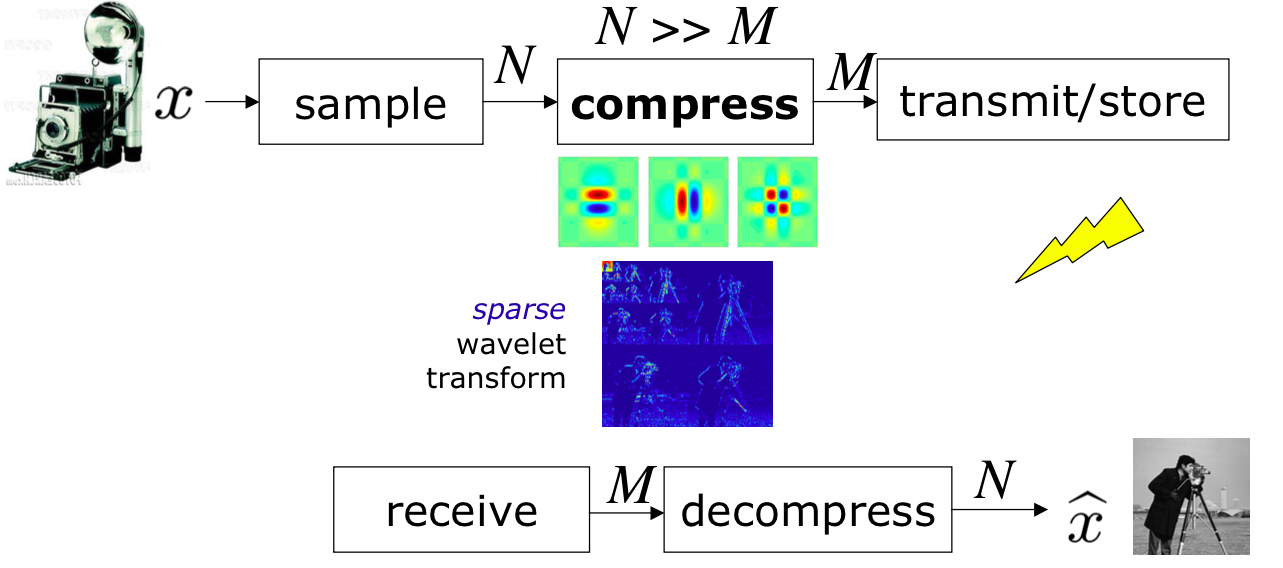
\includegraphics[width=5.0in]{figs/wavelets-arch.png}
%\DeclareGraphicsExtensions.
%\caption{An example of wavelet compression procedure. The camera first samples the image, and then analyses it using wavelets to compress and transmit. At the receiving end, the image is reconstructed.}
%\end{figure}


%---- contributes topics ----

%In order to solve these problems, this report studies novel approaches which respectively embed the CS framework into those systems. In our proposed CS-UWB system, random projection is located at transmitters to support CS framework while sub-Nyquist low-rate ADCs are implemented at receivers. As a result, not only the accuracy is improved but also the sampling cost is significantly reduced. On the other hand, we study the recent CS-CSS systems' performance and analyize the cost of embedding CS into such systems. The analysis result indicates us that rather than fully reconstructing the CS measurements, the partial recovery or extraction useful information directly from unrecovered signals is more attractive and suitable in many cognitive radio spectrum sensing cases since it improves the real-time capability while keeps low sampling rate in CS. This idea intrigues our future research directions and motivations aiming at compressive signal processing (CSP, including compressive measurements analysis and partial support recovery etc) for wideband signal processing in cognitive radios and ultra wideband systems.

%---- contributes summary ----

%\paragraph{Compressive digital filter and estimation:} Following the idea that signal recovery is not actually necessary in many signal processing applications, we broaden this result and demonstrate that random measurements can universally capture the information relevant for many CSP applications without any prior knowledge of either the signal class or the ultimate signal processing task. For instance, in [xx], a circulated matrix based filter paradigm is mathematically proved, which can directly extract useful information from compressive measurements without recovery. This idea can be embedded in many filter-bank needed designs then eliminate the existence of analog filter while implement the filter in digital domain. In this way, complexity and power cost can be saved.

%The detection, estimation, and classification tools we develop in this paper enable the system to perform these tasks much more efficiently in the compressive domain. Furthermore, the filtering procedure we describe facilitates the separation of signals after they have been acquired in the compressive domain so that each signal can be processed by the appropriate algorithm, depend- ing on the information sought by the user. 
